\begin{document}
Virtual Reality mag zwar relative neu auf dem Markt sein, jedoch ist die Technologie seit Jahrzehnten in der Entwicklung und es gab mehrere
Iterationen, welche verschiedene Versionen und Varianten der Technik für die virtuelle Welt hervorbrachte. \\ \\
Das Konzept der virtuellen Welt wurde vermutlich zum ersten mal im Jahre 1935 vom schriftsteller Stanley Weinbaum in der Science Fiction
Story Pygmalion's Spectacles beschrieben.\\ 
In dieser Geschichte schon, verwendete der Hauptcharakter, eine Brille um in eine virtuelle Welt zu gelangen, wo seine Handlungen
und Gefühle von und auf die reale Welt simuliert wurden. Dieses beschrieb relative akkurat welche Vorstellung und Visionen man hatte und im
Vergleich heutzutage feststellen und sehen wie sich diese Technologie entwickelte.\cite{virtualrealityhistory}\\ \\
Doch folgten eine reihe von Iterationen über die Jahrzehnte, welche den Werdegang der VR Brille von heute definierte. \\ \\
Somit wurde im Jahre 1956 von Morton Heilig die Senorama gebaut, welches die erste VR Maschine war. Es bündelte mehrere Technologien um alle
diesen Gerät gedreht und es wurde zu diesem Zeitpunkt als die Zukunft des Kinos betrachtet.\cite{virtualrealityhistory} \\
\begin{center}
    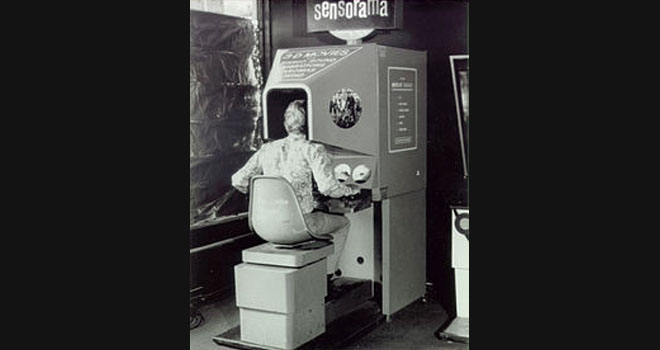
\includegraphics[width=0.75\textwidth]{sensorama-vr-machine.jpg}
\end{center}
\newpage \noindent
1960 veröffentlichte Heilig den ''Telesphere Mask'' welches das erste Head Mounted Display kurz HMD war. Es verfügte über die
Funktion der Ausgabe von 3D Bildern und hatte eine Stereo Ausgabe Möglichkeit. Dieses gerät verfügte jedoch noch nicht über die Funktion der
Bewegungsverfolgung, welche mit dem Gerät ''Headsight'' von Ceomeau und Bryen zwei Philco Corporation Ingenieuren kam. Es
verfügte über die Funktion der Bewegungsverfolgung des Kopfes, jedoch wurde dieses Gerät nicht als VR Brille verwendet sondern für das
Militär entwickelt welches sie in riskanten Regionen als fern Steuerung von Kameras verwendeten.\cite{virtualrealityhistory}\\
Ivan Sutherland welcher ein Informatiker in den Jahren 1965 war, veröffentlichte ein Paper namens Ultimate Display. In diesem beschrieb er
das Computer Hardware die virtuelle Welt erstellen und in Echtzeit verwalten sollte. Sein
\href{http://worrydream.com/refs/Sutherland%20-%20The%20Ultimate%20Display.pdf}{Paper} welches er veröffentliche wird als der Bauplan 
vom heutigen VR Brillen gesehen.\cite{virtualrealityhistory}\\
Von diesem Zeitpunkt an wurden die ersten HMD mit dem Fokus auf virtuelle Welten erfunden. Das gerät ''The Sword
of Damacles'' welches im Jahre 1968 erschien wurde, trotz seiner Fähigkeit 3D Modelnetze abhängig von der Perspektive des Benutzers
anzuzeigen, wegen seiner Größe und Notwendigkeit an einer Decke montiert zu sein nicht weiter als Labor Testphasen
entwickelt.\cite{virtualrealityhistory} \\
\begin{center}
    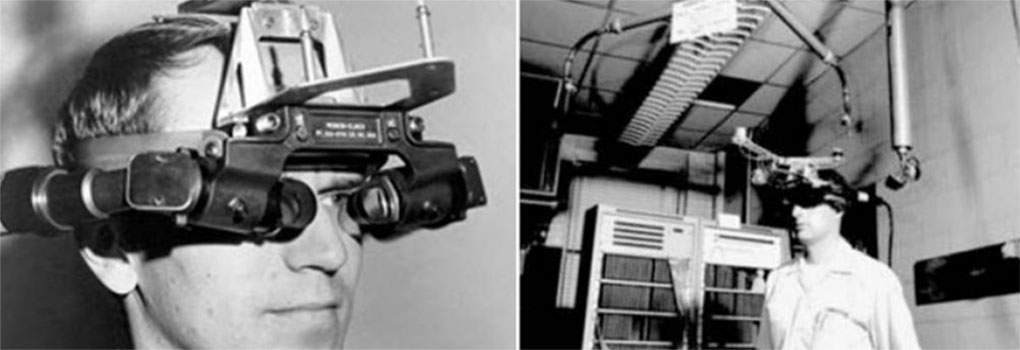
\includegraphics[width=0.75\textwidth]{sword-of-damacles.jpg}\cite{swordofdamacles}
\end{center}
Schon zu diesem Zeitpunkt erkannte man das man VR für Trainingsimulationen und Medizinischen Behandlungen verwenden kann. \\ 
Somit wurde schon im Jahre 1979 von McDonnel-Douglas Corporation eine HMD für den militärischen Gebrauch entwickelt, dieses Gerät war in der
lage die Augen des Benutzers verfolge um Bilder in Echtzeit passend zum Blickwinkel zu generieren.\cite{virtualrealityhistory}
\begin{center}
    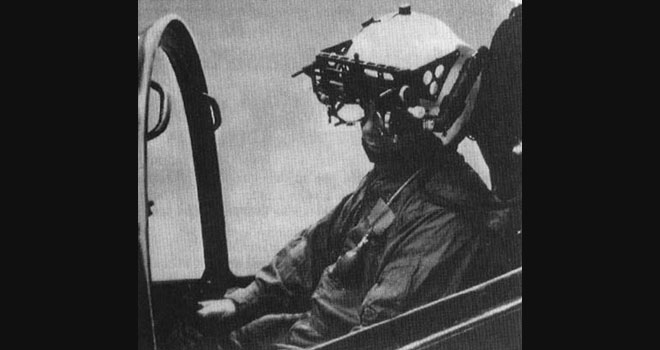
\includegraphics[width=0.5\textwidth]{VITAL-helmet-vr.jpg}\cite{vitalhelmet}
\end{center}
\newpage \noindent
Oder im Jahre 1989 von der Nasa um Austronauten für anhand von VR auszubilden.  
\begin{center}
    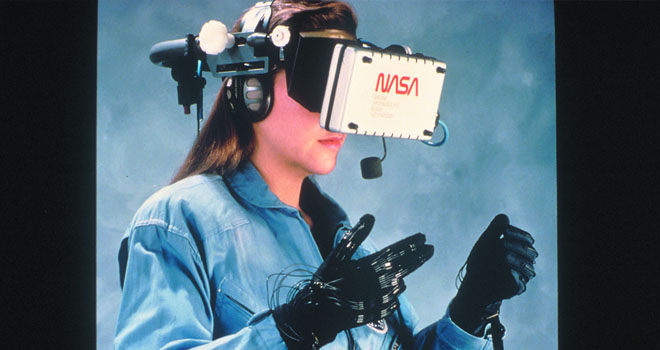
\includegraphics[width=0.5\textwidth]{virtual-environment-workstation-project-nasa.jpg}\cite{nasahelmet}
\end{center}
Einen Medizinischen gebraucht fand VR im Jahre 1997 durch Georgia Tech und Emory University welche den gebrauch von VR im Posttraumatischen
Belastungsstörungen für Veteranen erforschten. Hier wurden Kriegsszenarios simuliert welches Virtual Vietnam benannt wurde um diese Symptome
zu behandeln. Links zu Papern die zu dieser Behandlung veröffentlicht wurden.\cite{virtualrealityhistory}
\begin{center}
    \href{http://gotz.web.unc.edu/files/2013/10/icat.pdf}{Virtual Vietnam}
    \href{http://gotz.web.unc.edu/files/2013/10/jts1999.pdf}{Virtual Reality Exposure Therapy for PTSD}
\end{center}
Wenn man wieder auf den kommerziellen Verkauf von VR Brillen zurück kommt. Waren Jaron Lanier und Thomas Zimmerman, gründer von VPL Research
Inc., die ersten die VR Brillen, Handschuhe produzierten und für die Masse verkauften. Hierauf folgte bis auf den internen Gebrauch von VR
Technologien wie von der Nasa oder medizinischen Experimenten bis zum Jahre 2010 nichts neues.\cite{virtualrealityhistory} \\ \\
Palmer Luckey, erzeugte den ersten Prototypen für die Oculus Rift welcher den Entwicklungsdrang von VR Technologien wieder neu entfachte.  
Folgen tut eine Kickstarter Kampanie im Jahre 2012 welche 2.4 Millionen USD sammelte und die Produktion der Oculus Rift Brillen
in gang brachte.\\
Heutzutage hat jeder Hersteller (HTC, Sony, Apple, Google, Amazon, Samsung) seine eigenen VR Brillen und der Markt und Gebrauch von VR
variiert von der Industrie, Medizien, Bildung, Unterhaltung bis hin zur Forschung.\cite{virtualrealityhistory}
\end{document}
